\documentclass[1p]{elsarticle_modified}
%\bibliographystyle{elsarticle-num}

%\usepackage[colorlinks]{hyperref}
%\usepackage{abbrmath_seonhwa} %\Abb, \Ascr, \Acal ,\Abf, \Afrak
\usepackage{amsfonts}
\usepackage{amssymb}
\usepackage{amsmath}
\usepackage{amsthm}
\usepackage{scalefnt}
\usepackage{amsbsy}
\usepackage{kotex}
\usepackage{caption}
\usepackage{subfig}
\usepackage{color}
\usepackage{graphicx}
\usepackage{xcolor} %% white, black, red, green, blue, cyan, magenta, yellow
\usepackage{float}
\usepackage{setspace}
\usepackage{hyperref}

\usepackage{tikz}
\usetikzlibrary{arrows}

\usepackage{multirow}
\usepackage{array} % fixed length table
\usepackage{hhline}

%%%%%%%%%%%%%%%%%%%%%
\makeatletter
\renewcommand*\env@matrix[1][\arraystretch]{%
	\edef\arraystretch{#1}%
	\hskip -\arraycolsep
	\let\@ifnextchar\new@ifnextchar
	\array{*\c@MaxMatrixCols c}}
\makeatother %https://tex.stackexchange.com/questions/14071/how-can-i-increase-the-line-spacing-in-a-matrix
%%%%%%%%%%%%%%%

\usepackage[normalem]{ulem}

\newcommand{\msout}[1]{\ifmmode\text{\sout{\ensuremath{#1}}}\else\sout{#1}\fi}
%SOURCE: \msout is \stkout macro in https://tex.stackexchange.com/questions/20609/strikeout-in-math-mode

\newcommand{\cancel}[1]{
	\ifmmode
	{\color{red}\msout{#1}}
	\else
	{\color{red}\sout{#1}}
	\fi
}

\newcommand{\add}[1]{
	{\color{blue}\uwave{#1}}
}

\newcommand{\replace}[2]{
	\ifmmode
	{\color{red}\msout{#1}}{\color{blue}\uwave{#2}}
	\else
	{\color{red}\sout{#1}}{\color{blue}\uwave{#2}}
	\fi
}

\newcommand{\Sol}{\mathcal{S}} %segment
\newcommand{\D}{D} %diagram
\newcommand{\A}{\mathcal{A}} %arc


%%%%%%%%%%%%%%%%%%%%%%%%%%%%%5 test

\def\sl{\operatorname{\textup{SL}}(2,\Cbb)}
\def\psl{\operatorname{\textup{PSL}}(2,\Cbb)}
\def\quan{\mkern 1mu \triangleright \mkern 1mu}

\theoremstyle{definition}
\newtheorem{thm}{Theorem}[section]
\newtheorem{prop}[thm]{Proposition}
\newtheorem{lem}[thm]{Lemma}
\newtheorem{ques}[thm]{Question}
\newtheorem{cor}[thm]{Corollary}
\newtheorem{defn}[thm]{Definition}
\newtheorem{exam}[thm]{Example}
\newtheorem{rmk}[thm]{Remark}
\newtheorem{alg}[thm]{Algorithm}

\newcommand{\I}{\sqrt{-1}}
\begin{document}

%\begin{frontmatter}
%
%\title{Boundary parabolic representations of knots up to 8 crossings}
%
%%% Group authors per affiliation:
%\author{Yunhi Cho} 
%\address{Department of Mathematics, University of Seoul, Seoul, Korea}
%\ead{yhcho@uos.ac.kr}
%
%
%\author{Seonhwa Kim} %\fnref{s_kim}}
%\address{Center for Geometry and Physics, Institute for Basic Science, Pohang, 37673, Korea}
%\ead{ryeona17@ibs.re.kr}
%
%\author{Hyuk Kim}
%\address{Department of Mathematical Sciences, Seoul National University, Seoul 08826, Korea}
%\ead{hyukkim@snu.ac.kr}
%
%\author{Seokbeom Yoon}
%\address{Department of Mathematical Sciences, Seoul National University, Seoul, 08826,  Korea}
%\ead{sbyoon15@snu.ac.kr}
%
%\begin{abstract}
%We find all boundary parabolic representation of knots up to 8 crossings.
%
%\end{abstract}
%\begin{keyword}
%    \MSC[2010] 57M25 
%\end{keyword}
%
%\end{frontmatter}

%\linenumbers
%\tableofcontents
%
\newcommand\colored[1]{\textcolor{white}{\rule[-0.35ex]{0.8em}{1.4ex}}\kern-0.8em\color{red} #1}%
%\newcommand\colored[1]{\textcolor{white}{ #1}\kern-2.17ex	\textcolor{white}{ #1}\kern-1.81ex	\textcolor{white}{ #1}\kern-2.15ex\color{red}#1	}

{\Large $\underline{12a_{0735}~(K12a_{0735})}$}

\setlength{\tabcolsep}{10pt}
\renewcommand{\arraystretch}{1.6}
\vspace{1cm}\begin{tabular}{m{100pt}>{\centering\arraybackslash}m{274pt}}
\multirow{5}{120pt}{
	\centering
	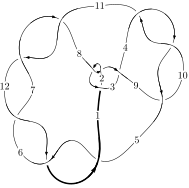
\includegraphics[width=112pt]{../../../GIT/diagram.site/Diagrams/png/1536_12a_0735.png}\\
\ \ \ A knot diagram\footnotemark}&
\allowdisplaybreaks
\textbf{Linearized knot diagam} \\
\cline{2-2}
 &
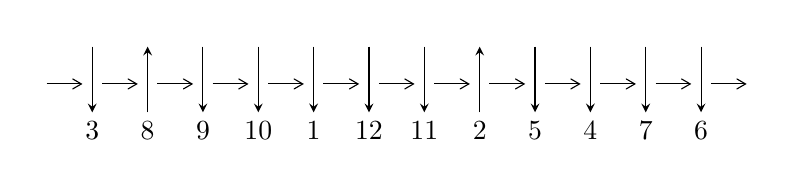
\begin{tikzpicture}[x=20pt, y=17pt]
	% nodes
	\node (C0) at (0, 0) {};
	\node (C1) at (1, 0) {};
	\node (C1U) at (1, +1) {};
	\node (C1D) at (1, -1) {3};

	\node (C2) at (2, 0) {};
	\node (C2U) at (2, +1) {};
	\node (C2D) at (2, -1) {8};

	\node (C3) at (3, 0) {};
	\node (C3U) at (3, +1) {};
	\node (C3D) at (3, -1) {9};

	\node (C4) at (4, 0) {};
	\node (C4U) at (4, +1) {};
	\node (C4D) at (4, -1) {10};

	\node (C5) at (5, 0) {};
	\node (C5U) at (5, +1) {};
	\node (C5D) at (5, -1) {1};

	\node (C6) at (6, 0) {};
	\node (C6U) at (6, +1) {};
	\node (C6D) at (6, -1) {12};

	\node (C7) at (7, 0) {};
	\node (C7U) at (7, +1) {};
	\node (C7D) at (7, -1) {11};

	\node (C8) at (8, 0) {};
	\node (C8U) at (8, +1) {};
	\node (C8D) at (8, -1) {2};

	\node (C9) at (9, 0) {};
	\node (C9U) at (9, +1) {};
	\node (C9D) at (9, -1) {5};

	\node (C10) at (10, 0) {};
	\node (C10U) at (10, +1) {};
	\node (C10D) at (10, -1) {4};

	\node (C11) at (11, 0) {};
	\node (C11U) at (11, +1) {};
	\node (C11D) at (11, -1) {7};

	\node (C12) at (12, 0) {};
	\node (C12U) at (12, +1) {};
	\node (C12D) at (12, -1) {6};
	\node (C13) at (13, 0) {};

	% arrows
	\draw[->,>={angle 60}]
	(C0) edge (C1) (C1) edge (C2) (C2) edge (C3) (C3) edge (C4) (C4) edge (C5) (C5) edge (C6) (C6) edge (C7) (C7) edge (C8) (C8) edge (C9) (C9) edge (C10) (C10) edge (C11) (C11) edge (C12) (C12) edge (C13) ;	\draw[->,>=stealth]
	(C1U) edge (C1D) (C2D) edge (C2U) (C3U) edge (C3D) (C4U) edge (C4D) (C5U) edge (C5D) (C6U) edge (C6D) (C7U) edge (C7D) (C8D) edge (C8U) (C9U) edge (C9D) (C10U) edge (C10D) (C11U) edge (C11D) (C12U) edge (C12D) ;
	\end{tikzpicture} \\
\hhline{~~} \\& 
\textbf{Solving Sequence} \\ \cline{2-2} 
 &
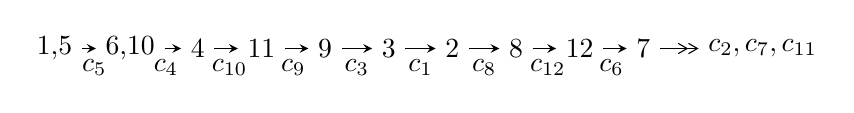
\begin{tikzpicture}[x=23pt, y=7pt]
	% node
	\node (A0) at (-1/8, 0) {1,5};
	\node (A1) at (17/16, 0) {6,10};
	\node (A2) at (17/8, 0) {4};
	\node (A3) at (25/8, 0) {11};
	\node (A4) at (33/8, 0) {9};
	\node (A5) at (41/8, 0) {3};
	\node (A6) at (49/8, 0) {2};
	\node (A7) at (57/8, 0) {8};
	\node (A8) at (65/8, 0) {12};
	\node (A9) at (73/8, 0) {7};
	\node (C1) at (1/2, -1) {$c_{5}$};
	\node (C2) at (13/8, -1) {$c_{4}$};
	\node (C3) at (21/8, -1) {$c_{10}$};
	\node (C4) at (29/8, -1) {$c_{9}$};
	\node (C5) at (37/8, -1) {$c_{3}$};
	\node (C6) at (45/8, -1) {$c_{1}$};
	\node (C7) at (53/8, -1) {$c_{8}$};
	\node (C8) at (61/8, -1) {$c_{12}$};
	\node (C9) at (69/8, -1) {$c_{6}$};
	\node (A10) at (11, 0) {$c_{2},c_{7},c_{11}$};

	% edge
	\draw[->,>=stealth]	
	(A0) edge (A1) (A1) edge (A2) (A2) edge (A3) (A3) edge (A4) (A4) edge (A5) (A5) edge (A6) (A6) edge (A7) (A7) edge (A8) (A8) edge (A9) ;
	\draw[->>,>={angle 60}]	
	(A9) edge (A10);
\end{tikzpicture} \\ 

\end{tabular} \\

\footnotetext{
The image of knot diagram is generated by the software ``\textbf{Draw programme}" developed by Andrew Bartholomew(\url{http://www.layer8.co.uk/maths/draw/index.htm\#Running-draw}), where we modified some parts for our purpose(\url{https://github.com/CATsTAILs/LinksPainter}).
}\phantom \\ \newline 
\centering \textbf{Ideals for irreducible components\footnotemark of $X_{\text{par}}$} 
 
\begin{align*}
I^u_{1}&=\langle 
2 u^{37}+2 u^{36}+\cdots+4 b+2,\;- u^{36}-23 u^{34}+\cdots+4 a-2,\;u^{38}+2 u^{37}+\cdots+5 u+2\rangle \\
I^u_{2}&=\langle 
2 u^4 a-2 u^3 a+a^2 u+5 u^2 a-4 a u+b+a+2 u-2,\\
\phantom{I^u_{2}}&\phantom{= \langle  }2 u^4 a^2- u^4 a+6 a^2 u^2+2 u^3 a-3 u^4+a^3-5 u^2 a+u^3+2 a^2+7 a u-10 u^2-2 a+3 u-5,\\
\phantom{I^u_{2}}&\phantom{= \langle  }u^5- u^4+4 u^3-3 u^2+3 u-1\rangle \\
I^u_{3}&=\langle 
u^3+b+2 u,\;- u^3- u^2+a-2 u-2,\;u^4+3 u^2+1\rangle \\
\\
\end{align*}
\raggedright * 3 irreducible components of $\dim_{\mathbb{C}}=0$, with total 57 representations.\\
\footnotetext{All coefficients of polynomials are rational numbers. But the coefficients are sometimes approximated in decimal forms when there is not enough margin.}
\newpage
\renewcommand{\arraystretch}{1}
\centering \section*{I. $I^u_{1}= \langle 2 u^{37}+2 u^{36}+\cdots+4 b+2,\;- u^{36}-23 u^{34}+\cdots+4 a-2,\;u^{38}+2 u^{37}+\cdots+5 u+2 \rangle$}
\flushleft \textbf{(i) Arc colorings}\\
\begin{tabular}{m{7pt} m{180pt} m{7pt} m{180pt} }
\flushright $a_{1}=$&$\begin{pmatrix}0\\u\end{pmatrix}$ \\
\flushright $a_{5}=$&$\begin{pmatrix}1\\0\end{pmatrix}$ \\
\flushright $a_{6}=$&$\begin{pmatrix}1\\u^2\end{pmatrix}$ \\
\flushright $a_{10}=$&$\begin{pmatrix}\frac{1}{4} u^{36}+\frac{23}{4} u^{34}+\cdots+\frac{5}{2} u+\frac{1}{2}\\-\frac{1}{2} u^{37}-\frac{1}{2} u^{36}+\cdots-\frac{1}{4} u-\frac{1}{2}\end{pmatrix}$ \\
\flushright $a_{4}=$&$\begin{pmatrix}\frac{1}{4} u^{33}+5 u^{31}+\cdots-\frac{1}{4} u+1\\-\frac{1}{4} u^{33}-\frac{21}{4} u^{31}+\cdots-\frac{1}{2} u^2-\frac{1}{2} u\end{pmatrix}$ \\
\flushright $a_{11}=$&$\begin{pmatrix}u^3+2 u\\u^5+3 u^3+u\end{pmatrix}$ \\
\flushright $a_{9}=$&$\begin{pmatrix}-\frac{1}{2} u^{37}-\frac{1}{4} u^{36}+\cdots+\frac{1}{4} u^2+\frac{9}{4} u\\-\frac{1}{2} u^{37}-\frac{1}{2} u^{36}+\cdots-\frac{1}{4} u-\frac{1}{2}\end{pmatrix}$ \\
\flushright $a_{3}=$&$\begin{pmatrix}-\frac{1}{2} u^{37}- u^{36}+\cdots-\frac{15}{4} u-2\\-\frac{3}{4} u^{33}-\frac{3}{4} u^{32}+\cdots-\frac{1}{2} u-1\end{pmatrix}$ \\
\flushright $a_{2}=$&$\begin{pmatrix}\frac{1}{4} u^{32}+\frac{21}{4} u^{30}+\cdots-\frac{1}{2} u-\frac{1}{2}\\\frac{1}{4} u^{32}+5 u^{30}+\cdots+\frac{5}{4} u^2+u\end{pmatrix}$ \\
\flushright $a_{8}=$&$\begin{pmatrix}u^4+3 u^2+1\\u^6+4 u^4+3 u^2\end{pmatrix}$ \\
\flushright $a_{12}=$&$\begin{pmatrix}u\\u^3+u\end{pmatrix}$ \\
\flushright $a_{7}=$&$\begin{pmatrix}u^2+1\\u^4+2 u^2\end{pmatrix}$\\&\end{tabular}
\flushleft \textbf{(ii) Obstruction class $= -1$}\\~\\
\flushleft \textbf{(iii) Cusp Shapes $= -2 u^{37}-4 u^{36}+\cdots-4 u-14$}\\~\\
\newpage\renewcommand{\arraystretch}{1}
\flushleft \textbf{(iv) u-Polynomials at the component}\newline \\
\begin{tabular}{m{50pt}|m{274pt}}
Crossings & \hspace{64pt}u-Polynomials at each crossing \\
\hline $$\begin{aligned}c_{1}\end{aligned}$$&$\begin{aligned}
&u^{38}+17 u^{37}+\cdots+194 u+25
\end{aligned}$\\
\hline $$\begin{aligned}c_{2},c_{8}\end{aligned}$$&$\begin{aligned}
&u^{38}- u^{37}+\cdots-6 u+5
\end{aligned}$\\
\hline $$\begin{aligned}c_{3}\end{aligned}$$&$\begin{aligned}
&u^{38}-2 u^{37}+\cdots+400 u+800
\end{aligned}$\\
\hline $$\begin{aligned}c_{4},c_{9},c_{10}\end{aligned}$$&$\begin{aligned}
&u^{38}- u^{37}+\cdots-4 u+5
\end{aligned}$\\
\hline $$\begin{aligned}c_{5},c_{6},c_{7}\\c_{11},c_{12}\end{aligned}$$&$\begin{aligned}
&u^{38}-2 u^{37}+\cdots-5 u+2
\end{aligned}$\\
\hline
\end{tabular}\\~\\
\newpage\renewcommand{\arraystretch}{1}
\flushleft \textbf{(v) Riley Polynomials at the component}\newline \\
\begin{tabular}{m{50pt}|m{274pt}}
Crossings & \hspace{64pt}Riley Polynomials at each crossing \\
\hline $$\begin{aligned}c_{1}\end{aligned}$$&$\begin{aligned}
&y^{38}+13 y^{37}+\cdots+8514 y+625
\end{aligned}$\\
\hline $$\begin{aligned}c_{2},c_{8}\end{aligned}$$&$\begin{aligned}
&y^{38}+17 y^{37}+\cdots+194 y+25
\end{aligned}$\\
\hline $$\begin{aligned}c_{3}\end{aligned}$$&$\begin{aligned}
&y^{38}-6 y^{37}+\cdots+7276800 y+640000
\end{aligned}$\\
\hline $$\begin{aligned}c_{4},c_{9},c_{10}\end{aligned}$$&$\begin{aligned}
&y^{38}+37 y^{37}+\cdots+34 y+25
\end{aligned}$\\
\hline $$\begin{aligned}c_{5},c_{6},c_{7}\\c_{11},c_{12}\end{aligned}$$&$\begin{aligned}
&y^{38}+48 y^{37}+\cdots+19 y+4
\end{aligned}$\\
\hline
\end{tabular}\\~\\
\newpage\flushleft \textbf{(vi) Complex Volumes and Cusp Shapes}
$$\begin{array}{c|c|c}  
\text{Solutions to }I^u_{1}& \I (\text{vol} + \sqrt{-1}CS) & \text{Cusp shape}\\
 \hline 
\begin{aligned}
u &= -0.339832 + 0.921512 I \\
a &= \phantom{-}0.416428 + 0.809179 I \\
b &= \phantom{-}0.816368 - 0.218889 I\end{aligned}
 & -0.53116 + 6.72152 I & -6.76982 - 7.69269 I \\ \hline\begin{aligned}
u &= -0.339832 - 0.921512 I \\
a &= \phantom{-}0.416428 - 0.809179 I \\
b &= \phantom{-}0.816368 + 0.218889 I\end{aligned}
 & -0.53116 - 6.72152 I & -6.76982 + 7.69269 I \\ \hline\begin{aligned}
u &= -0.325570 + 0.993591 I \\
a &= -1.55595 - 1.85235 I \\
b &= -0.257004 + 1.389260 I\end{aligned}
 & \phantom{-}7.06845 + 5.49844 I & \phantom{-}0.54907 - 4.52833 I \\ \hline\begin{aligned}
u &= -0.325570 - 0.993591 I \\
a &= -1.55595 + 1.85235 I \\
b &= -0.257004 - 1.389260 I\end{aligned}
 & \phantom{-}7.06845 - 5.49844 I & \phantom{-}0.54907 + 4.52833 I \\ \hline\begin{aligned}
u &= \phantom{-}0.394709 + 0.970581 I \\
a &= \phantom{-}1.66954 - 1.57123 I \\
b &= \phantom{-}0.33472 + 1.39633 I\end{aligned}
 & \phantom{-}4.59569 - 10.87090 I & -2.77827 + 8.43141 I \\ \hline\begin{aligned}
u &= \phantom{-}0.394709 - 0.970581 I \\
a &= \phantom{-}1.66954 + 1.57123 I \\
b &= \phantom{-}0.33472 - 1.39633 I\end{aligned}
 & \phantom{-}4.59569 + 10.87090 I & -2.77827 - 8.43141 I \\ \hline\begin{aligned}
u &= -0.009913 + 0.916024 I \\
a &= -0.106232 + 0.617839 I \\
b &= -0.435699 - 0.647770 I\end{aligned}
 & \phantom{-}2.92919 - 1.46585 I & -0.29190 + 4.46440 I \\ \hline\begin{aligned}
u &= -0.009913 - 0.916024 I \\
a &= -0.106232 - 0.617839 I \\
b &= -0.435699 + 0.647770 I\end{aligned}
 & \phantom{-}2.92919 + 1.46585 I & -0.29190 - 4.46440 I \\ \hline\begin{aligned}
u &= -0.091063 + 1.155310 I \\
a &= -0.37132 - 2.12708 I \\
b &= -0.03930 + 1.42339 I\end{aligned}
 & \phantom{-}9.62190 + 2.62526 I & \phantom{-}1.76254 - 3.39036 I \\ \hline\begin{aligned}
u &= -0.091063 - 1.155310 I \\
a &= -0.37132 + 2.12708 I \\
b &= -0.03930 - 1.42339 I\end{aligned}
 & \phantom{-}9.62190 - 2.62526 I & \phantom{-}1.76254 + 3.39036 I\\
 \hline 
 \end{array}$$\newpage$$\begin{array}{c|c|c}  
\text{Solutions to }I^u_{1}& \I (\text{vol} + \sqrt{-1}CS) & \text{Cusp shape}\\
 \hline 
\begin{aligned}
u &= \phantom{-}0.475449 + 0.649846 I \\
a &= -0.634708 + 0.373029 I \\
b &= \phantom{-}0.237413 - 1.333010 I\end{aligned}
 & \phantom{-}2.66568 + 3.67725 I & -3.88495 - 1.85217 I \\ \hline\begin{aligned}
u &= \phantom{-}0.475449 - 0.649846 I \\
a &= -0.634708 - 0.373029 I \\
b &= \phantom{-}0.237413 + 1.333010 I\end{aligned}
 & \phantom{-}2.66568 - 3.67725 I & -3.88495 + 1.85217 I \\ \hline\begin{aligned}
u &= -0.326550 + 0.707311 I \\
a &= \phantom{-}0.365685 + 0.985287 I \\
b &= \phantom{-}0.598316 + 0.079539 I\end{aligned}
 & -1.81820 - 0.62723 I & -9.78117 - 0.63046 I \\ \hline\begin{aligned}
u &= -0.326550 - 0.707311 I \\
a &= \phantom{-}0.365685 - 0.985287 I \\
b &= \phantom{-}0.598316 - 0.079539 I\end{aligned}
 & -1.81820 + 0.62723 I & -9.78117 + 0.63046 I \\ \hline\begin{aligned}
u &= -0.453897 + 0.489215 I \\
a &= \phantom{-}0.911640 + 0.461033 I \\
b &= -0.076008 - 1.314890 I\end{aligned}
 & \phantom{-}4.18206 + 0.81384 I & -1.66334 - 4.28381 I \\ \hline\begin{aligned}
u &= -0.453897 - 0.489215 I \\
a &= \phantom{-}0.911640 - 0.461033 I \\
b &= -0.076008 + 1.314890 I\end{aligned}
 & \phantom{-}4.18206 - 0.81384 I & -1.66334 + 4.28381 I \\ \hline\begin{aligned}
u &= \phantom{-}0.634985 + 0.149850 I \\
a &= -1.313290 - 0.234988 I \\
b &= -0.296893 - 1.359070 I\end{aligned}
 & \phantom{-}1.15622 - 7.39365 I & -7.23665 + 6.75615 I \\ \hline\begin{aligned}
u &= \phantom{-}0.634985 - 0.149850 I \\
a &= -1.313290 + 0.234988 I \\
b &= -0.296893 + 1.359070 I\end{aligned}
 & \phantom{-}1.15622 + 7.39365 I & -7.23665 - 6.75615 I \\ \hline\begin{aligned}
u &= -0.551325 + 0.214770 I \\
a &= \phantom{-}1.406100 - 0.007220 I \\
b &= \phantom{-}0.191390 - 1.321750 I\end{aligned}
 & \phantom{-}3.34928 + 2.52485 I & -4.06452 - 3.23642 I \\ \hline\begin{aligned}
u &= -0.551325 - 0.214770 I \\
a &= \phantom{-}1.406100 + 0.007220 I \\
b &= \phantom{-}0.191390 + 1.321750 I\end{aligned}
 & \phantom{-}3.34928 - 2.52485 I & -4.06452 + 3.23642 I\\
 \hline 
 \end{array}$$\newpage$$\begin{array}{c|c|c}  
\text{Solutions to }I^u_{1}& \I (\text{vol} + \sqrt{-1}CS) & \text{Cusp shape}\\
 \hline 
\begin{aligned}
u &= -0.556094 + 0.096366 I \\
a &= -1.338990 + 0.086931 I \\
b &= -0.729346 + 0.157605 I\end{aligned}
 & -3.64092 + 3.67836 I & -13.1775 - 5.2178 I \\ \hline\begin{aligned}
u &= -0.556094 - 0.096366 I \\
a &= -1.338990 - 0.086931 I \\
b &= -0.729346 - 0.157605 I\end{aligned}
 & -3.64092 - 3.67836 I & -13.1775 + 5.2178 I \\ \hline\begin{aligned}
u &= \phantom{-}0.06495 + 1.55948 I \\
a &= \phantom{-}0.124474 - 1.120870 I \\
b &= -0.146346 + 1.269640 I\end{aligned}
 & \phantom{-}9.94200 + 1.81077 I & \phantom{-0.000000 } 0 \\ \hline\begin{aligned}
u &= \phantom{-}0.06495 - 1.55948 I \\
a &= \phantom{-}0.124474 + 1.120870 I \\
b &= -0.146346 - 1.269640 I\end{aligned}
 & \phantom{-}9.94200 - 1.81077 I & \phantom{-0.000000 } 0 \\ \hline\begin{aligned}
u &= \phantom{-}0.232971 + 0.274282 I \\
a &= \phantom{-}0.783127 + 0.921776 I \\
b &= \phantom{-}0.170162 + 0.354512 I\end{aligned}
 & -0.605257 - 0.910546 I & -10.00383 + 7.24439 I \\ \hline\begin{aligned}
u &= \phantom{-}0.232971 - 0.274282 I \\
a &= \phantom{-}0.783127 - 0.921776 I \\
b &= \phantom{-}0.170162 - 0.354512 I\end{aligned}
 & -0.605257 + 0.910546 I & -10.00383 - 7.24439 I \\ \hline\begin{aligned}
u &= -0.05271 + 1.63939 I \\
a &= -0.104717 - 0.802437 I \\
b &= -0.537806 + 0.097751 I\end{aligned}
 & \phantom{-}6.35089 + 0.56961 I & \phantom{-0.000000 } 0 \\ \hline\begin{aligned}
u &= -0.05271 - 1.63939 I \\
a &= -0.104717 + 0.802437 I \\
b &= -0.537806 - 0.097751 I\end{aligned}
 & \phantom{-}6.35089 - 0.56961 I & \phantom{-0.000000 } 0 \\ \hline\begin{aligned}
u &= -0.01436 + 1.69488 I \\
a &= -0.095169 - 0.847455 I \\
b &= \phantom{-}0.572206 + 0.761360 I\end{aligned}
 & \phantom{-}12.20970 - 1.29201 I & \phantom{-0.000000 } 0 \\ \hline\begin{aligned}
u &= -0.01436 - 1.69488 I \\
a &= -0.095169 + 0.847455 I \\
b &= \phantom{-}0.572206 - 0.761360 I\end{aligned}
 & \phantom{-}12.20970 + 1.29201 I & \phantom{-0.000000 } 0\\
 \hline 
 \end{array}$$\newpage$$\begin{array}{c|c|c}  
\text{Solutions to }I^u_{1}& \I (\text{vol} + \sqrt{-1}CS) & \text{Cusp shape}\\
 \hline 
\begin{aligned}
u &= -0.08704 + 1.69484 I \\
a &= -0.001733 - 0.692432 I \\
b &= -0.884556 + 0.249985 I\end{aligned}
 & \phantom{-}8.67383 + 8.38204 I & \phantom{-0.000000 } 0 \\ \hline\begin{aligned}
u &= -0.08704 - 1.69484 I \\
a &= -0.001733 + 0.692432 I \\
b &= -0.884556 - 0.249985 I\end{aligned}
 & \phantom{-}8.67383 - 8.38204 I & \phantom{-0.000000 } 0 \\ \hline\begin{aligned}
u &= \phantom{-}0.10617 + 1.70777 I \\
a &= -1.09920 + 1.99516 I \\
b &= -0.36348 - 1.42519 I\end{aligned}
 & \phantom{-}14.0039 - 12.8731 I & \phantom{-0.000000 } 0 \\ \hline\begin{aligned}
u &= \phantom{-}0.10617 - 1.70777 I \\
a &= -1.09920 - 1.99516 I \\
b &= -0.36348 + 1.42519 I\end{aligned}
 & \phantom{-}14.0039 + 12.8731 I & \phantom{-0.000000 } 0 \\ \hline\begin{aligned}
u &= -0.08545 + 1.71485 I \\
a &= \phantom{-}1.00730 + 2.20606 I \\
b &= \phantom{-}0.29380 - 1.43752 I\end{aligned}
 & \phantom{-}16.6465 + 7.1508 I & \phantom{-0.000000 } 0 \\ \hline\begin{aligned}
u &= -0.08545 - 1.71485 I \\
a &= \phantom{-}1.00730 - 2.20606 I \\
b &= \phantom{-}0.29380 + 1.43752 I\end{aligned}
 & \phantom{-}16.6465 - 7.1508 I & \phantom{-0.000000 } 0 \\ \hline\begin{aligned}
u &= -0.01542 + 1.74340 I \\
a &= \phantom{-}0.18700 + 2.55613 I \\
b &= \phantom{-}0.05206 - 1.51390 I\end{aligned}
 & -19.4879 + 3.0073 I & \phantom{-0.000000 } 0 \\ \hline\begin{aligned}
u &= -0.01542 - 1.74340 I \\
a &= \phantom{-}0.18700 - 2.55613 I \\
b &= \phantom{-}0.05206 + 1.51390 I\end{aligned}
 & -19.4879 - 3.0073 I & \phantom{-0.000000 } 0\\
 \hline 
 \end{array}$$\newpage\newpage\renewcommand{\arraystretch}{1}
\centering \section*{II. $I^u_{2}= \langle 2 u^4 a-2 u^3 a+\cdots+a-2,\;2 u^4 a^2- u^4 a+\cdots-2 a-5,\;u^5- u^4+4 u^3-3 u^2+3 u-1 \rangle$}
\flushleft \textbf{(i) Arc colorings}\\
\begin{tabular}{m{7pt} m{180pt} m{7pt} m{180pt} }
\flushright $a_{1}=$&$\begin{pmatrix}0\\u\end{pmatrix}$ \\
\flushright $a_{5}=$&$\begin{pmatrix}1\\0\end{pmatrix}$ \\
\flushright $a_{6}=$&$\begin{pmatrix}1\\u^2\end{pmatrix}$ \\
\flushright $a_{10}=$&$\begin{pmatrix}a\\-2 u^4 a+2 u^3 a- a^2 u-5 u^2 a+4 a u- a-2 u+2\end{pmatrix}$ \\
\flushright $a_{4}=$&$\begin{pmatrix}- u^4 a- a^2 u^2+u^3 a+2 u^4-4 u^2 a-2 u^3- a^2+a u+6 u^2- a-4 u+4\\- u^4 a^2-2 a^2 u^2-2 u^4+2 u^3+3 a u-4 u^2-2 a+4 u\end{pmatrix}$ \\
\flushright $a_{11}=$&$\begin{pmatrix}u^3+2 u\\u^4- u^3+3 u^2-2 u+1\end{pmatrix}$ \\
\flushright $a_{9}=$&$\begin{pmatrix}-2 u^4 a+2 u^3 a- a^2 u-5 u^2 a+4 a u-2 u+2\\-2 u^4 a+2 u^3 a- a^2 u-5 u^2 a+4 a u- a-2 u+2\end{pmatrix}$ \\
\flushright $a_{3}=$&$\begin{pmatrix}- u^3 a^2-2 u^4 a+\cdots-3 a+4\\- u^4 a^2-4 u^4+\cdots+a^2-3 a\end{pmatrix}$ \\
\flushright $a_{2}=$&$\begin{pmatrix}u^4 a^2+u^4 a+3 a^2 u^2- u^3 a+4 u^2 a+a^2-4 a u-2 u^2+3 a-4\\u^4 a^2+2 a^2 u^2+2 u^4-2 u^3-3 a u+4 u^2+2 a-4 u\end{pmatrix}$ \\
\flushright $a_{8}=$&$\begin{pmatrix}u^4+3 u^2+1\\u^4- u^3+3 u^2-2 u+1\end{pmatrix}$ \\
\flushright $a_{12}=$&$\begin{pmatrix}u\\u^3+u\end{pmatrix}$ \\
\flushright $a_{7}=$&$\begin{pmatrix}u^2+1\\u^4+2 u^2\end{pmatrix}$\\&\end{tabular}
\flushleft \textbf{(ii) Obstruction class $= -1$}\\~\\
\flushleft \textbf{(iii) Cusp Shapes $= -4 u^4+4 u^3-16 u^2+12 u-14$}\\~\\
\newpage\renewcommand{\arraystretch}{1}
\flushleft \textbf{(iv) u-Polynomials at the component}\newline \\
\begin{tabular}{m{50pt}|m{274pt}}
Crossings & \hspace{64pt}u-Polynomials at each crossing \\
\hline $$\begin{aligned}c_{1}\end{aligned}$$&$\begin{aligned}
&u^{15}+10 u^{14}+\cdots+3 u-1
\end{aligned}$\\
\hline $$\begin{aligned}c_{2},c_{4},c_{8}\\c_{9},c_{10}\end{aligned}$$&$\begin{aligned}
&u^{15}+5 u^{13}+\cdots+u+1
\end{aligned}$\\
\hline $$\begin{aligned}c_{3}\end{aligned}$$&$\begin{aligned}
&(u^5+u^4- u^2+u+1)^3
\end{aligned}$\\
\hline $$\begin{aligned}c_{5},c_{6},c_{7}\\c_{11},c_{12}\end{aligned}$$&$\begin{aligned}
&(u^5+u^4+4 u^3+3 u^2+3 u+1)^3
\end{aligned}$\\
\hline
\end{tabular}\\~\\
\newpage\renewcommand{\arraystretch}{1}
\flushleft \textbf{(v) Riley Polynomials at the component}\newline \\
\begin{tabular}{m{50pt}|m{274pt}}
Crossings & \hspace{64pt}Riley Polynomials at each crossing \\
\hline $$\begin{aligned}c_{1}\end{aligned}$$&$\begin{aligned}
&y^{15}-10 y^{14}+\cdots+15 y-1
\end{aligned}$\\
\hline $$\begin{aligned}c_{2},c_{4},c_{8}\\c_{9},c_{10}\end{aligned}$$&$\begin{aligned}
&y^{15}+10 y^{14}+\cdots+3 y-1
\end{aligned}$\\
\hline $$\begin{aligned}c_{3}\end{aligned}$$&$\begin{aligned}
&(y^5- y^4+4 y^3-3 y^2+3 y-1)^3
\end{aligned}$\\
\hline $$\begin{aligned}c_{5},c_{6},c_{7}\\c_{11},c_{12}\end{aligned}$$&$\begin{aligned}
&(y^5+7 y^4+16 y^3+13 y^2+3 y-1)^3
\end{aligned}$\\
\hline
\end{tabular}\\~\\
\newpage\flushleft \textbf{(vi) Complex Volumes and Cusp Shapes}
$$\begin{array}{c|c|c}  
\text{Solutions to }I^u_{2}& \I (\text{vol} + \sqrt{-1}CS) & \text{Cusp shape}\\
 \hline 
\begin{aligned}
u &= \phantom{-}0.233677 + 0.885557 I \\
a &= -0.323874 + 0.796296 I \\
b &= -0.638808 - 0.271585 I\end{aligned}
 & \phantom{-}1.81981 - 2.21397 I & -3.11432 + 4.22289 I \\ \hline\begin{aligned}
u &= \phantom{-}0.233677 + 0.885557 I \\
a &= -0.156756 + 0.463494 I \\
b &= \phantom{-}0.435133 - 0.988544 I\end{aligned}
 & \phantom{-}1.81981 - 2.21397 I & -3.11432 + 4.22289 I \\ \hline\begin{aligned}
u &= \phantom{-}0.233677 + 0.885557 I \\
a &= \phantom{-}2.13619 - 2.53516 I \\
b &= \phantom{-}0.203675 + 1.260130 I\end{aligned}
 & \phantom{-}1.81981 - 2.21397 I & -3.11432 + 4.22289 I \\ \hline\begin{aligned}
u &= \phantom{-}0.233677 - 0.885557 I \\
a &= -0.323874 - 0.796296 I \\
b &= -0.638808 + 0.271585 I\end{aligned}
 & \phantom{-}1.81981 + 2.21397 I & -3.11432 - 4.22289 I \\ \hline\begin{aligned}
u &= \phantom{-}0.233677 - 0.885557 I \\
a &= -0.156756 - 0.463494 I \\
b &= \phantom{-}0.435133 + 0.988544 I\end{aligned}
 & \phantom{-}1.81981 + 2.21397 I & -3.11432 - 4.22289 I \\ \hline\begin{aligned}
u &= \phantom{-}0.233677 - 0.885557 I \\
a &= \phantom{-}2.13619 + 2.53516 I \\
b &= \phantom{-}0.203675 - 1.260130 I\end{aligned}
 & \phantom{-}1.81981 + 2.21397 I & -3.11432 - 4.22289 I \\ \hline\begin{aligned}
u &= \phantom{-}0.416284\phantom{ +0.000000I} \\
a &= \phantom{-}1.12253\phantom{ +0.000000I} \\
b &= \phantom{-}0.511430\phantom{ +0.000000I}\end{aligned}
 & -0.882183\phantom{ +0.000000I} & -11.6090\phantom{ +0.000000I} \\ \hline\begin{aligned}
u &= \phantom{-}0.416284\phantom{ +0.000000I} \\
a &= -2.11117 + 0.66665 I \\
b &= -0.255715 + 1.093700 I\end{aligned}
 & -0.882183\phantom{ +0.000000I} & -11.6090\phantom{ +0.000000I} \\ \hline\begin{aligned}
u &= \phantom{-}0.416284\phantom{ +0.000000I} \\
a &= -2.11117 - 0.66665 I \\
b &= -0.255715 - 1.093700 I\end{aligned}
 & -0.882183\phantom{ +0.000000I} & -11.6090\phantom{ +0.000000I} \\ \hline\begin{aligned}
u &= \phantom{-}0.05818 + 1.69128 I \\
a &= \phantom{-}0.154896 - 0.889970 I \\
b &= -0.549193 + 1.000850 I\end{aligned}
 & \phantom{-}10.95830 - 3.33174 I & -2.08126 + 2.36228 I\\
 \hline 
 \end{array}$$\newpage$$\begin{array}{c|c|c}  
\text{Solutions to }I^u_{2}& \I (\text{vol} + \sqrt{-1}CS) & \text{Cusp shape}\\
 \hline 
\begin{aligned}
u &= \phantom{-}0.05818 + 1.69128 I \\
a &= -0.007493 - 0.744869 I \\
b &= \phantom{-}0.762735 + 0.344098 I\end{aligned}
 & \phantom{-}10.95830 - 3.33174 I & -2.08126 + 2.36228 I \\ \hline\begin{aligned}
u &= \phantom{-}0.05818 + 1.69128 I \\
a &= -1.25306 + 2.70311 I \\
b &= -0.213543 - 1.344950 I\end{aligned}
 & \phantom{-}10.95830 - 3.33174 I & -2.08126 + 2.36228 I \\ \hline\begin{aligned}
u &= \phantom{-}0.05818 - 1.69128 I \\
a &= \phantom{-}0.154896 + 0.889970 I \\
b &= -0.549193 - 1.000850 I\end{aligned}
 & \phantom{-}10.95830 + 3.33174 I & -2.08126 - 2.36228 I \\ \hline\begin{aligned}
u &= \phantom{-}0.05818 - 1.69128 I \\
a &= -0.007493 + 0.744869 I \\
b &= \phantom{-}0.762735 - 0.344098 I\end{aligned}
 & \phantom{-}10.95830 + 3.33174 I & -2.08126 - 2.36228 I \\ \hline\begin{aligned}
u &= \phantom{-}0.05818 - 1.69128 I \\
a &= -1.25306 - 2.70311 I \\
b &= -0.213543 + 1.344950 I\end{aligned}
 & \phantom{-}10.95830 + 3.33174 I & -2.08126 - 2.36228 I\\
 \hline 
 \end{array}$$\newpage\newpage\renewcommand{\arraystretch}{1}
\centering \section*{III. $I^u_{3}= \langle u^3+b+2 u,\;- u^3- u^2+a-2 u-2,\;u^4+3 u^2+1 \rangle$}
\flushleft \textbf{(i) Arc colorings}\\
\begin{tabular}{m{7pt} m{180pt} m{7pt} m{180pt} }
\flushright $a_{1}=$&$\begin{pmatrix}0\\u\end{pmatrix}$ \\
\flushright $a_{5}=$&$\begin{pmatrix}1\\0\end{pmatrix}$ \\
\flushright $a_{6}=$&$\begin{pmatrix}1\\u^2\end{pmatrix}$ \\
\flushright $a_{10}=$&$\begin{pmatrix}u^3+u^2+2 u+2\\- u^3-2 u\end{pmatrix}$ \\
\flushright $a_{4}=$&$\begin{pmatrix}u^3+3 u\\1\end{pmatrix}$ \\
\flushright $a_{11}=$&$\begin{pmatrix}u^3+2 u\\0\end{pmatrix}$ \\
\flushright $a_{9}=$&$\begin{pmatrix}u^2+2\\- u^3-2 u\end{pmatrix}$ \\
\flushright $a_{3}=$&$\begin{pmatrix}u^3+3 u\\1\end{pmatrix}$ \\
\flushright $a_{2}=$&$\begin{pmatrix}u^3+3 u\\u+1\end{pmatrix}$ \\
\flushright $a_{8}=$&$\begin{pmatrix}0\\- u^2-1\end{pmatrix}$ \\
\flushright $a_{12}=$&$\begin{pmatrix}u\\u^3+u\end{pmatrix}$ \\
\flushright $a_{7}=$&$\begin{pmatrix}u^2+1\\- u^2-1\end{pmatrix}$\\&\end{tabular}
\flushleft \textbf{(ii) Obstruction class $= 1$}\\~\\
\flushleft \textbf{(iii) Cusp Shapes $= -4$}\\~\\
\newpage\renewcommand{\arraystretch}{1}
\flushleft \textbf{(iv) u-Polynomials at the component}\newline \\
\begin{tabular}{m{50pt}|m{274pt}}
Crossings & \hspace{64pt}u-Polynomials at each crossing \\
\hline $$\begin{aligned}c_{1}\end{aligned}$$&$\begin{aligned}
&(u-1)^4
\end{aligned}$\\
\hline $$\begin{aligned}c_{2},c_{4},c_{8}\\c_{9},c_{10}\end{aligned}$$&$\begin{aligned}
&(u^2+1)^2
\end{aligned}$\\
\hline $$\begin{aligned}c_{3}\end{aligned}$$&$\begin{aligned}
&u^4
\end{aligned}$\\
\hline $$\begin{aligned}c_{5},c_{6},c_{7}\\c_{11},c_{12}\end{aligned}$$&$\begin{aligned}
&u^4+3 u^2+1
\end{aligned}$\\
\hline
\end{tabular}\\~\\
\newpage\renewcommand{\arraystretch}{1}
\flushleft \textbf{(v) Riley Polynomials at the component}\newline \\
\begin{tabular}{m{50pt}|m{274pt}}
Crossings & \hspace{64pt}Riley Polynomials at each crossing \\
\hline $$\begin{aligned}c_{1}\end{aligned}$$&$\begin{aligned}
&(y-1)^4
\end{aligned}$\\
\hline $$\begin{aligned}c_{2},c_{4},c_{8}\\c_{9},c_{10}\end{aligned}$$&$\begin{aligned}
&(y+1)^4
\end{aligned}$\\
\hline $$\begin{aligned}c_{3}\end{aligned}$$&$\begin{aligned}
&y^4
\end{aligned}$\\
\hline $$\begin{aligned}c_{5},c_{6},c_{7}\\c_{11},c_{12}\end{aligned}$$&$\begin{aligned}
&(y^2+3 y+1)^2
\end{aligned}$\\
\hline
\end{tabular}\\~\\
\newpage\flushleft \textbf{(vi) Complex Volumes and Cusp Shapes}
$$\begin{array}{c|c|c}  
\text{Solutions to }I^u_{3}& \I (\text{vol} + \sqrt{-1}CS) & \text{Cusp shape}\\
 \hline 
\begin{aligned}
u &= \phantom{-0.000000 -}0.618034 I \\
a &= \phantom{-}1.61803 + 1.00000 I \\
b &= \phantom{-0.000000 } -1.000000 I\end{aligned}
 & \phantom{-}0.986960\phantom{ +0.000000I} & -4.00000\phantom{ +0.000000I} \\ \hline\begin{aligned}
u &= \phantom{-0.000000 } -0.618034 I \\
a &= \phantom{-}1.61803 - 1.00000 I \\
b &= \phantom{-0.000000 -}1.000000 I\end{aligned}
 & \phantom{-}0.986960\phantom{ +0.000000I} & -4.00000\phantom{ +0.000000I} \\ \hline\begin{aligned}
u &= \phantom{-0.000000 -}1.61803 I \\
a &= -0.618034 - 1.000000 I \\
b &= \phantom{-0.000000 -}1.000000 I\end{aligned}
 & \phantom{-}8.88264\phantom{ +0.000000I} & -4.00000\phantom{ +0.000000I} \\ \hline\begin{aligned}
u &= \phantom{-0.000000 } -1.61803 I \\
a &= -0.618034 + 1.000000 I \\
b &= \phantom{-0.000000 } -1.000000 I\end{aligned}
 & \phantom{-}8.88264\phantom{ +0.000000I} & -4.00000\phantom{ +0.000000I}\\
 \hline 
 \end{array}$$\newpage
\newpage\renewcommand{\arraystretch}{1}
\centering \section*{ IV. u-Polynomials}
\begin{tabular}{m{50pt}|m{274pt}}
Crossings & \hspace{64pt}u-Polynomials at each crossing \\
\hline $$\begin{aligned}c_{1}\end{aligned}$$&$\begin{aligned}
&((u-1)^4)(u^{15}+10 u^{14}+\cdots+3 u-1)(u^{38}+17 u^{37}+\cdots+194 u+25)
\end{aligned}$\\
\hline $$\begin{aligned}c_{2},c_{8}\end{aligned}$$&$\begin{aligned}
&((u^2+1)^2)(u^{15}+5 u^{13}+\cdots+u+1)(u^{38}- u^{37}+\cdots-6 u+5)
\end{aligned}$\\
\hline $$\begin{aligned}c_{3}\end{aligned}$$&$\begin{aligned}
&u^4(u^5+u^4- u^2+u+1)^3(u^{38}-2 u^{37}+\cdots+400 u+800)
\end{aligned}$\\
\hline $$\begin{aligned}c_{4},c_{9},c_{10}\end{aligned}$$&$\begin{aligned}
&((u^2+1)^2)(u^{15}+5 u^{13}+\cdots+u+1)(u^{38}- u^{37}+\cdots-4 u+5)
\end{aligned}$\\
\hline $$\begin{aligned}c_{5},c_{6},c_{7}\\c_{11},c_{12}\end{aligned}$$&$\begin{aligned}
&(u^4+3 u^2+1)(u^5+u^4+\cdots+3 u+1)^{3}(u^{38}-2 u^{37}+\cdots-5 u+2)
\end{aligned}$\\
\hline
\end{tabular}\newpage\renewcommand{\arraystretch}{1}
\centering \section*{ V. Riley Polynomials}
\begin{tabular}{m{50pt}|m{274pt}}
Crossings & \hspace{64pt}Riley Polynomials at each crossing \\
\hline $$\begin{aligned}c_{1}\end{aligned}$$&$\begin{aligned}
&((y-1)^4)(y^{15}-10 y^{14}+\cdots+15 y-1)\\
&\cdot(y^{38}+13 y^{37}+\cdots+8514 y+625)
\end{aligned}$\\
\hline $$\begin{aligned}c_{2},c_{8}\end{aligned}$$&$\begin{aligned}
&((y+1)^4)(y^{15}+10 y^{14}+\cdots+3 y-1)(y^{38}+17 y^{37}+\cdots+194 y+25)
\end{aligned}$\\
\hline $$\begin{aligned}c_{3}\end{aligned}$$&$\begin{aligned}
&y^4(y^5- y^4+4 y^3-3 y^2+3 y-1)^3\\
&\cdot(y^{38}-6 y^{37}+\cdots+7276800 y+640000)
\end{aligned}$\\
\hline $$\begin{aligned}c_{4},c_{9},c_{10}\end{aligned}$$&$\begin{aligned}
&((y+1)^4)(y^{15}+10 y^{14}+\cdots+3 y-1)(y^{38}+37 y^{37}+\cdots+34 y+25)
\end{aligned}$\\
\hline $$\begin{aligned}c_{5},c_{6},c_{7}\\c_{11},c_{12}\end{aligned}$$&$\begin{aligned}
&(y^2+3 y+1)^2(y^5+7 y^4+16 y^3+13 y^2+3 y-1)^3\\
&\cdot(y^{38}+48 y^{37}+\cdots+19 y+4)
\end{aligned}$\\
\hline
\end{tabular}
\vskip 2pc
\end{document}